\documentclass{standalone}
\usepackage{tikz}
\usepackage{verbatim}
\usetikzlibrary{positioning}
\begin{document}
\pagestyle{empty}
  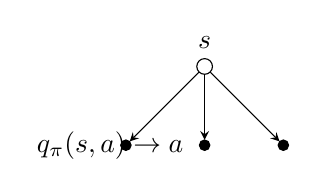
\begin{tikzpicture}
    \node[draw,circle,scale=0.6] (s) at (0,0) {};
    \node[above=1mm] {$s$};
    \foreach \x in {-1, 0, 1} {
      \node[draw,circle,fill,scale=0.4] (b\x) at (\x, -1) {};
      \draw[-stealth] (s) -- (b\x);
    }
    \node at (-1.2, -1) {$q_{\pi}(s,a) \rightarrow a$};
  \end{tikzpicture}
\end{document}